\chapter{Event Reconstruction and Monte Carlo Simulations}
After data is collected it undergoes 'Event Reconstruction'.
At this stage %particles
%a series of algorithm to identify and particles and event variables

\section{Track and Primary Vertex Reconstruction}
%%%%%%%%%%%%%%%%Track Reconstruction [31] %TRK-11-001
One of the central design motivations to CMS%fix
is a multi-layer tracker with a low occupancy, high granularity
inner silicon pixel detector and a lower granularity silicon strip detector.
%For the Wbb cross section measurement each event is associated
%to a primary vertex, muons are
%and each jet is required to contain a secondary vertex.
%In the search for a MSSM higgs it is association with a primary vertex
%is also required and tracks are used to identify taus, muons, jets, whatelse?
%These characteristics %cause
%complex algorithms to be developed primarily based on Kalman
%Filter algorithms and 
%write an intro
%Track selection involves selection of tracks which are consistent with being produced promptly in the primary interaction region by imposing requirements on the maximum value of significance of the transverse impact parameter relative to the beam spot
\subsection{Track Reconstruction}
In a technique known as Combined Track Finding (CTF),
the collection of reconstructed tracks is produced via
multiple iterations of the CTF track reconstruction sequence.
The first three iterations are meant to reconstruct successively
lower $p_{T}$ and quality tracks.%%not quite right actually...
%while iterations four through six recover any tracks 
%not found by previous iterations.

After each iteration the CTF track reconstruction sequence, the hits
associated with tracks are removed; this reduces the combinatorial complexity
and simplifies subsequent iterations in a search for more difficult classes of track (for example,
low $p_{t}$ or which are greatly displaced).
The CTF track reconstruction proceeds as follows:
\begin{itemize}
\item First, seeds are generated which provides the initial track candidates.
Charged particles follow helical paths in the magnetic field therefore five parameters (including curvature)
are needed to define a trajectory; to determine these five parameters at least
3 hits or 2 hits in the pixel detector and a constraint on the origin of the track trajectory from the beam
spot is required. Seeds are built in the inner part of the tracker
and track candidates are reconstructed outwards. This is due to a higher finer granularity 
and hence lower occupancy in the center of the pixel detector. Each iteration of CTF
uses independent quality parameters for seeding layers. 
\item Next, track finding is performed based on the Kalman filter method \cite{KalmanFilter}.
Track finding starts by using the seed trajectories to define and then search
for adjacent layers of the detector with a hit. The next step provides the possibility
of adding an invalid hit in the case where the particle failed to produce a hit.
Finally the track finding algorithm updates the trajectories of the tracks. 
%track fitting by means of kalman filter and smoother
\item Track fitting then is used to adjust for the possibility of bias added during the track
finding stage. The trajectory is therefore refitted using a Kalman filter and smoother with
a Runge-Kutta propagator that takes into account both material effect and accomodates
for a inhomogeneous magnetic field.
%track selection sets quality flags and discards tracks that fail certain criteria
\item The final step is track selection where tracks are required to pass a number of quality
based selection criteria. 
The selection criteria puts a requirement on a track's number of layers %fix
with valid hits, the fit-based $\chi^{2}/dof$, and the track's compatibility
with a primary vertex (PV). In addition to these, several requirements are
imposed as a function of track $p_{T}$, $\eta$, and the number of layers
with valid hits. 
\end{itemize}
The tracks and primary vertices found with this algorithm are known as pixel 
tracks and pixel vertices, respectively. The performance of the track reconstruction
offline software is shown in figure \ref{fig:TrackerPerformance}.
\begin{figure}[t]
  \centering
 \begin{subfigure}[b]{.4\textwidth}
	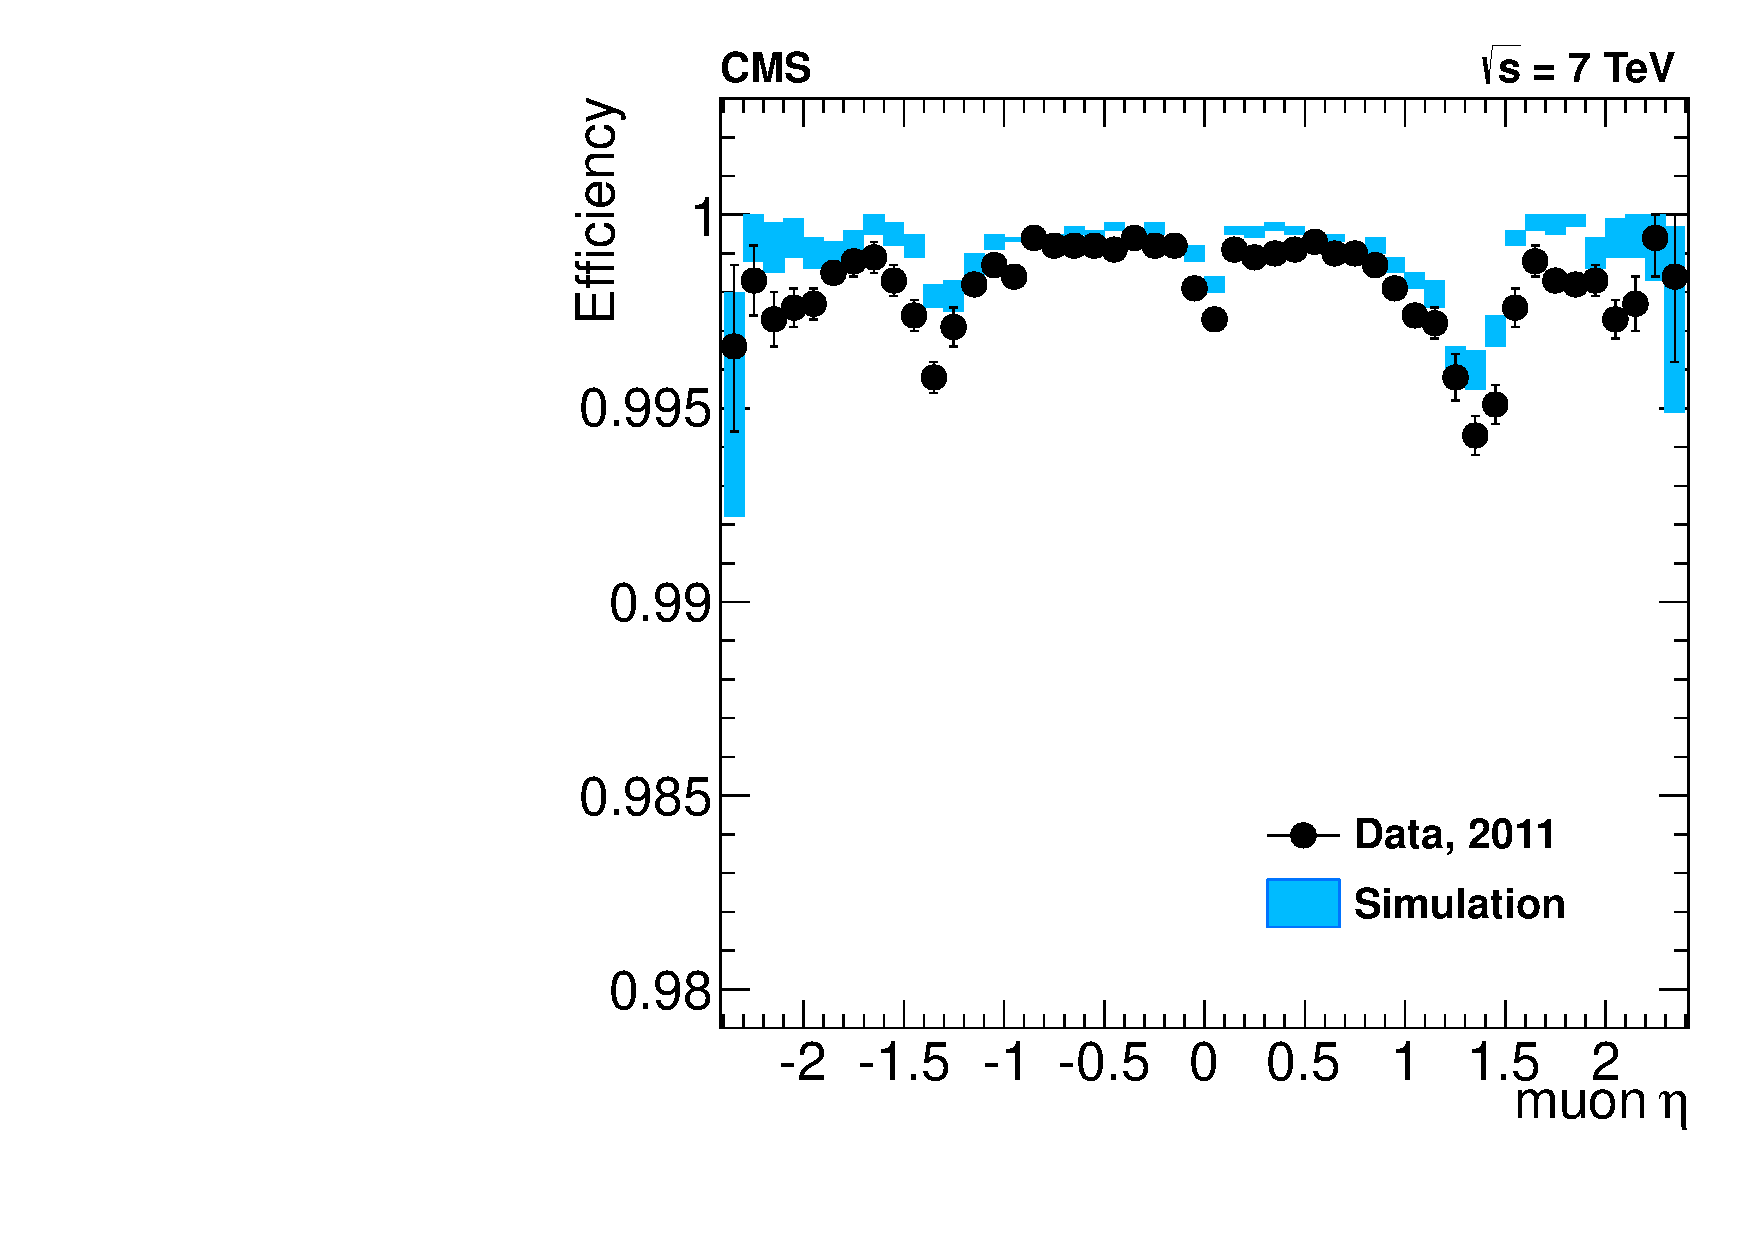
\includegraphics[width=\textwidth]{images/TrackerEffEta.pdf}
  \end{subfigure}
  \begin{subfigure}[b]{.4\textwidth}
	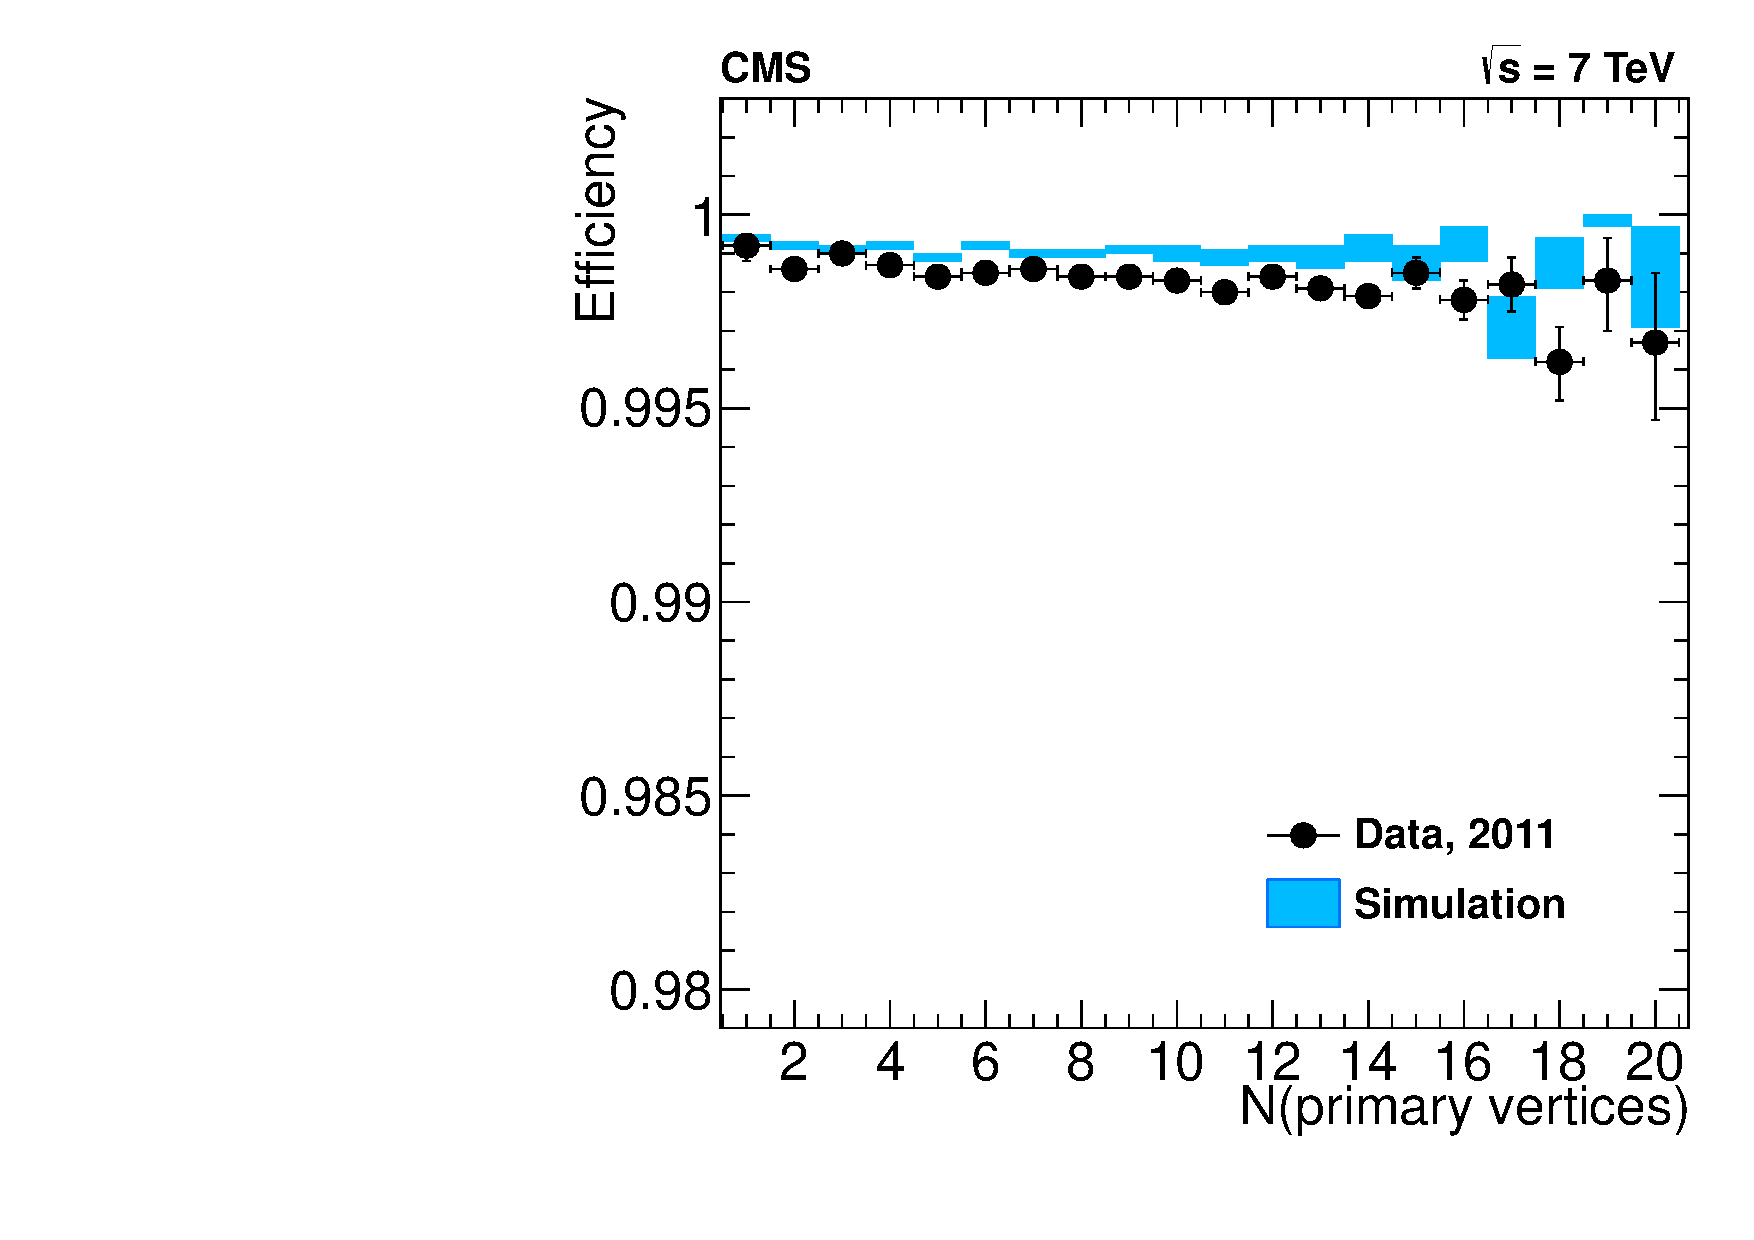
\includegraphics[width=\textwidth]{images/TrackerEffVtx.pdf}
  \end{subfigure}
  	\caption[Tracker Performance]
   	{Tracker efficiency of muons in $Z\rightarrow\mu\mu$ decays. Measured using Tag and Probe as a function of $\eta$ (left) and number of vertices (right)}
	\label{fig:TrackerPerformance}
\end{figure}
\subsection{Primary Vertex Reconstrucion}
Primary vertices (PVs) are reconstruct in order to locate and determine the associated uncertainty of all
proton-proton interaction vertices regardless of whether it is a 'signal' or 'background' vertex.
Primary vertex reconstruction proceeds in three steps.

The first step is to select tracks based on their association with a primary interaction region.
To do this, a number of quality selections are imposed: they are based upon the significance of the
transverse impact parameter ($d_{xy}$), the number of strip and pixel hits that are 
associated with a track and the normalized $\chi^{2}$ from the fit to the
trajectory. In selecting tracks their is no requirement on the $p_{T}$ of the track; 
this is important so that all PVs including ones from minimum bias events will be reconstructed.

The second step is to cluster the selected tracks based on their $z$ coodinate at their
point of closest approach to the beam spot. This is done using a Deterministic Annealing (DA)
algorithm which finds a global minimum given many degrees of freedom.%%ref DA, More on DA?

The third and final step is to take candidate vertices based on DA clustering in $z$ and use
an 'adaptive vertex fitter' %ref
to compute vertex parameters. These parameters include the 3-D position and covariance matrix,
as well as indicators for the success of the fit such as the number of degrees ($n_{dof}$) of freedom for
each vertex and weights of the track used in each vertex. The adaptive vertex fitter
uses a modified definition of $n_{dof}$ where,
\begin{equation}
n_{dof} = -3+2\sum^{nTracks}_{i=1} w_{i},
\end{equation}
Here, $w_{i}$ is the weight of the $i^{th}$ track. This implies that $n_{dof}$ is strongly
correlated with the number of tracks that are compatible with arising from the interaction
region which means that $n_{dof}$ can be also be used to select true proton-proton interactions.
%Vertex reconstruction [33], [34] 
\section{Electron ID and Reconstruction}
%Ecal Seeding or track seeding??

%GSF[38]

% Rejection of Electrons from converted photons [39]

%electron ID ---twiki table

%Electron trigger?? maybe
\section{Muon ID and Reconstruction}
Muons at CMS are reconstructed using information from both the 
tracker and the muon detectors. 
%In Wbb high pt muons
%in h to tautau soft muons used.
%Muon reco [40]
\subsection{Standalone Muon Reconstruction}
Standalone $\mu$ reconstruction uses only tracks from the muon system
to reconstruct tracks using a kalman filter technique which is seeded
by track segments or Level-1 trigger electronics. Tracks are propagated
in iterative steps taking into account the magnetic field, muon energy loss in the material,
multiple scattering and missing hits in the muon system.
Next a suitable $\chi^{2}$ cut is applied to reject bad hits due to showering,
delta rays and pair production. A backward Kalman filter is then applied,
working from outside in and finally the track is extrapolated to the 
beam-spot and a vertex-constrained fit to the track
parameters is performed.
\subsection{Global Muon Reconstruction}
Global muon reconstruction matches standalone tracks to tracks in the tracking
system. 
Tracks are selected which roughly correspond in momentum and position to 
the standalone muon tracks. This is performed in two steps: First,
tracks are selected in a defined $\eta\times\phi$ region which is centered
on the standalone track. Next, spatial and momentum matching is 
used to select the best matching track. Compatibility of the standalone track and tracker tarck with the
primary vertex is also required. Finally a new 'global track' is created combining
tracker and muon hits; at this stage, no new hits are selected, instead, 
the selected hits are refitted as a global track. If more than one candidate
track pair is matched then the candidate with the best $\chi^{2}$ value
is selected. 
For muons with $p_{T}<200\GeV$ the $p_{T}$ measurement is driven
by the fantastic tracker resoluion.
%In muons with a higher $p_{T}$, as might be found
%in the boosted topology of $\Wbb$ it is useful to requir
\subsection{Tracker Muon Reconstruction}

%Muon ID (use old muon plots?) mention muon veto in analysis

%Muon trigger

%\section on PF??
% section on lepton isolation?

\section{$\tau$ ID and Reconstruction}
The $\tau$ lepton's high mass means that the $\tau$ plays a very important
roll in search for the SM higgs boson, and MSSM higgs bosons.
The life time of the $\tau$ is short enough that they decay before reaching the inner
most detector. This short lifetime makes $\tau$ reconstruction particularly challenging;
the solution is to reconstruct the decay products of the $\tau$. 

The dominant hadronic $\tau$ decays ($\tau_{h}$) are outlined in table %%%insert table.
These decays consist of one or three charged $\pi$ mesons and up to two $\pi^{0}$ mesons.
This thesis uses the hadron plus strips (HPS) algorithm for the reconstruction of
hadronic $\tau$'s. %%%%ref tau id paper
The HPS algorithm takes into account photon conversions in the CMS tracker
material. %the electron positron decays will bend in the magnetic field
therefore %the HPS algorithm, say something about PF particles
reconstructs photons into 'strips' which are objects which are built%fix
out of electromagnetic particle particles within a window of size $\delta\eta=0.05$
and $\delta\phi=0.20$. The algorithm starts by centering a strip on the
most energetic electromagnetic particle within the PF jet, next it searches
for other electromagnetic particles within the window. If another electromagnetic
particle is found then the object gets associated with the strip and
the four-momentum is recalculated. This procedure is repeated until no other
particles are found. Strips which satisfy the requirement of $\p_{t}^{strip}>1GeV/c$
are finally combined with the charged hadrons to reconstruct individual
$\tau_{h}$ decay modes.

The following decay topologies are considered by the HPS $\tau$ ID algorithm:%%write list
\item Single Hadron reconstructs the $h^{-}$ and $h^{-}\pi^{0}$
\item
\item
\item
Charged hadrons and strips are required to be contained within a cone
of size $\delta R=(2.8\GeV/p_{T}^{\tau_{h}})$ where $p_{T}^{\tau_{h}$ is 
the transverse momentum of the $\tau$ hadron $p_{T}^{\tau_{h}$ is 
required to match the $(\eta,\phi)$ direction of the original PF jet within
a radius of $\delta R=0.1$. 
%%four momenta must match decay modes
%50-200 MeV for pi0, 0.3 to 1.3 GeV for \rho
%and 0.8 to 1.5 GeV for $a_{1}$

%%%%Tau Isolation from paper
%%%Tau performance plots

\section{Jet ID and Reconstruction}
%Particle flow
%Anti-Kt algo [43]
The primary motive behind choosing the Anti-$k_{T}$ algorithm is that it is both


%Jet energy corrections [44]
\subsection{b-Jet ID}
%CSV algorithm
%SV in jets
\section{Missing Transverse Energy}
%met 
%any documentation